% --------------------------------------------------------------------------- %
% Poster for the ECCS 2011 Conference about Elementary Dynamic Networks.      %
% --------------------------------------------------------------------------- %
% Created with Brian Amberg's LaTeX Poster Template. Please refer for the     %
% attached README.md file for the details how to compile with `pdflatex`.     %
% --------------------------------------------------------------------------- %
% $LastChangedDate:: 2011-09-11 10:57:12 +0200 (V, 11 szept. 2011)          $ %
% $LastChangedRevision:: 128                                                $ %
% $LastChangedBy:: rlegendi                                                 $ %
% $Id:: poster.tex 128 2011-09-11 08:57:12Z rlegendi                        $ %
% --------------------------------------------------------------------------- %
\documentclass[a0paper,landscape]{baposter}

\usepackage{relsize}		% For \smaller
\usepackage{url}			% For \url
% \usepackage{epstopdf}	% Included EPS files automatically converted to PDF to include with pdflatex
\usepackage{blindtext}
\usepackage{geometry}
 \geometry{
 top=7mm,
 left=5mm,
 right=7mm
 }

%% Define path for figures -- for safety, keep the last /
\graphicspath{{/your/figure/directory/here/if/any/}
{/an/second/directory/path/can/go/here/}}
\usepackage{pstricks}
\usepackage{amsmath,amssymb,amsthm,slashed,graphicx}
\newtheorem{thm}{Theorem}
\newtheorem{defn}{Definition}
\newtheorem{lemma}{Lemma}
\newtheorem{cor}{Corollary}

\usepackage{biblatex}
\addbibresource{citation.bib}
%%% Global Settings %%%%%%%%%%%%%%%%%%%%%%%%%%%%%%%%%%%%%%%%%%%%%%%%%%%%%%%%%%%

\graphicspath{{pix/}}	% Root directory of the pictures 
% \tracingstats=2			% Enabled LaTeX logging with conditionals
\usepackage{tikz}
%%% Color Definitions %%%%%%%%%%%%%%%%%%%%%%%%%%%%%%%%%%%%%%%%%%%%%%%%%%%%%%%%%

\definecolor{bordercol}{RGB}{88,44,131}
\definecolor{headercol1}{RGB}{88,44,131}
\definecolor{headercol2}{RGB}{88,44,131}
\definecolor{headerfontcol}{RGB}{255,255,255}
\definecolor{boxcolor}{RGB}{255,255,255}

%%%%%%%%%%%%%%%%%%%%%%%%%%%%%%%%%%%%%%%%%%%%%%%%%%%%%%%%%%%%%%%%%%%%%%%%%%%%%%%%
%%% Utility functions %%%%%%%%%%%%%%%%%%%%%%%%%%%%%%%%%%%%%%%%%%%%%%%%%%%%%%%%%%

%%% Save space in lists. Use this after the opening of the list %%%%%%%%%%%%%%%%
\newcommand{\compresslist}{
	\setlength{\itemsep}{1pt}
	\setlength{\parskip}{0pt}
	\setlength{\parsep}{0pt}
}


\usepackage{lipsum}
\usepackage{multicol}
%\setlength{\columnseprule}{0.4pt}
\setlength{\tabcolsep}{30pt}
%%%%%%%%%%%%%%%%%%%%%%%%%%%%%%%%%%%%%%%%%%%%%%%%%%%%%%%%%%%%%%%%%%%%%%%%%%%%%%%
%%% Document Start %%%%%%%%%%%%%%%%%%%%%%%%%%%%%%%%%%%%%%%%%%%%%%%%%%%%%%%%%%%%
%%%%%%%%%%%%%%%%%%%%%%%%%%%%%%%%%%%%%%%%%%%%%%%%%%%%%%%%%%%%%%%%%%%%%%%%%%%%%%%

\begin{document}
\typeout{Poster rendering started}

%%% Setting Background Image %%%%%%%%%%%%%%%%%%%%%%%%%%%%%%%%%%%%%%%%%%%%%%%%%%
\background{
	\begin{tikzpicture}[remember picture,overlay]%
	% \draw (current page.north west)+(-2em,2em) node[anchor=north west]
	% {\includegraphics[height=1.1\textheight]{background}};
	\end{tikzpicture}
}


\makeatletter
\renewcommand{\baposter@box@headerdrawtext@rectangle}[1]{
  \path (\baposter@box@name nw) +(0.5\boxwidth,-0.5\baposter@box@@boxheaderheight) node[anchor=center] {#1};%
}
\makeatother
%%% General Poster Settings %%%%%%%%%%%%%%%%%%%%%%%%%%%%%%%%%%%%%%%%%%%%%%%%%%%
%%%%%% Eye Catcher, Title, Authors and University Images %%%%%%%%%%%%%%%%%%%%%%
\begin{poster}{
	grid=false,
	% Option is left on true though the eyecatcher is not used. The reason is
	% that we have a bit nicer looking title and author formatting in the headercol
	% this way
	%eyecatcher=false, 
	borderColor=bordercol,
	headerColorOne=headercol1,
	headerColorTwo=headercol2,
	headerFontColor=headerfontcol,
	% Only simple background color used, no shading, so boxColorTwo isn't necessary
	boxColorOne=boxcolor,
	headershape=rectangle,
	headerfont=\Large\sf\bf\Centering,
	textborder=,
	background=user,
	headerborder=open,
    boxshade=plain
}
%%% Eye Cacther %%%%%%%%%%%%%%%%%%%%%%%%%%%%%%%%%%%%%%%%%%%%%%%%%%%%%%%%%%%%%%%
% {
% 	Eye Catcher, empty if option eyecatcher=false - unused
% }
{
% The logos are compressed a bit into a simple box to make them smaller on the result
% (Wasn't able to find any bigger of them.)
\setlength\fboxsep{0pt}
\setlength\fboxrule{0pt}
	\fbox{
		\begin{minipage}{14em}
			
\includegraphics[scale=0.1]{tcu_logo.png}
		\end{minipage}
	}
}
%%% Title %%%%%%%%%%%%%%%%%%%%%%%%%%%%%%%%%%%%%%%%%%%%%%%%%%%%%%%%%%%%%%%%%%%%%
{\bf
 \smaller Estimation of Misclassification Rates \\ for Human and AI Reading Accuracy Measurements
}
%%% Authors %%%%%%%%%%%%%%%%%%%%%%%%%%%%%%%%%%%%%%%%%%%%%%%%%%%%%%%%%%%%%%%%%%%
{
	Ngoc Vu \hspace{2cm} Advisor: Dr. Nelis Potgieter\\
	{\smaller \textit{Department of Mathematics, Texas Christian University, Fort Worth, Texas}}
}
%%% Logo %%%%%%%%%%%%%%%%%%%%%%%%%%%%%%%%%%%%%%%%%%%%%%%%%%%%%%%%%%%%%%%%%%%%%%
{
% The logos are compressed a bit into a simple box to make them smaller on the result
% (Wasn't able to find any bigger of them.)
\setlength\fboxsep{0pt}
\setlength\fboxrule{0pt}
	\fbox{
		\begin{minipage}{14em}
			
\includegraphics[width=11em,height=6em]{scicom-logo.jpg}
		\end{minipage}
	}
}



\headerbox{Introduction}{name=intro, span=1,column=0}{
Oral Reading Accuracy is an important measure of reading proficiency. Traditionally scored by human observers, recently AI systems integrating voice recognition software have also been utilized, see Nese et al (2015). This study develops two statistical models to evaluate the efficacy of technology in ORA assessment. The goal is to estimate the true positive and true negative rates associated with different scoring methods.}

\headerbox{Data Description}{name=data,span=1,column=1}{

The ORA data was collected from a sample of 507 elementary school students. Each student was assigned one of ten study passages of different length and difficulty.  Both human and AI evaluations recorded the WRC score. Figure 1 and Table 1 below illustrate the observed scores ($Y_1$ and $Y_2$) against the gold-standard score $X$ for each student.\smallskip

\begin{center}
 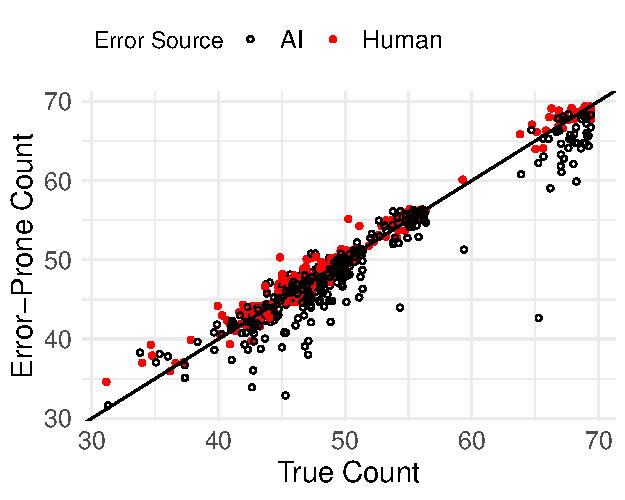
\includegraphics[width=\linewidth]{scatter_v2.pdf}
  \captionof{Figure 1: }{Comparison of True and Error-Prone \\ Counts in ORA Assessment: Human vs. AI.}   
\end{center}
\smallskip
  
In Figure 1, human scores (red) cluster more closely to the reference line, indicating greater rating consistency. Furthermore, AI scores (black) are much more likely to fall below the reference line, indicating bias introduced by automatic scoring.

\begin{center}
    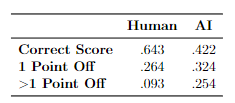
\includegraphics[width=.7\linewidth]{sum_table2.png}\\ 
    \captionof{Table 1: }{Accuracy Proportions:\\ True vs Error-Prone WRC}
\end{center}

Although human evaluators show evidence of greater consistency, this rating methods require more time and effort. Therefore, we are interested in understanding and addressing the errors of AI systems for further improvements in WRC measurement. 
}

\headerbox{Model Illustration}{name=model,span=1,column=2}{

Here are two scenarios illustrating the impact of incorrect counts. With $(\boldsymbol{\pi_{tp},\pi_{tn})=(0.95,0.65)}$, the distribution shifts leftward, yielding a lower mean and inflated standard deviation. Parameters $(\boldsymbol{\pi_{tp},\pi_{tn})=(0.99,0.05)}$ result in a rightward shift, producing a higher mean and reduced standard deviation.

\vspace{-0.75\baselineskip}
\begin{center}
    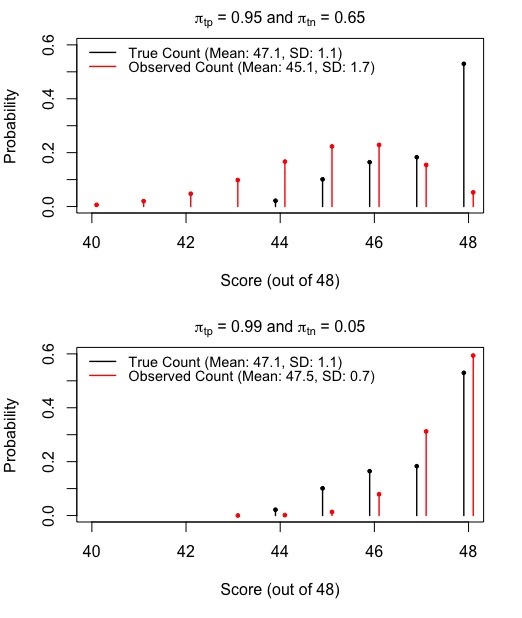
\includegraphics[width=0.95\linewidth]{two_pmf_examples.jpeg}\\
    \captionof{Figure 2: }{Illustrating the Error Effect}
\end{center}
}

\headerbox{Complete Data Solution}{name=sol,span=1,column=2,below=model}{

Our solution assumes access to gold-standard measurements $X$ alongside error-prone data $Y$. From binomial distribution properties, we have moment relationships
\vspace{-0.5\baselineskip}
\begin{center}
\fbox{
$$\mu_y = E[Y] = \mu_x \cdot \pi_{tp} + (N-\mu_x) \cdot (1-\pi_{tn})$$}
\end{center}
\vspace{-0.5\baselineskip}
and
\vspace{-0.5\baselineskip}
\begin{center}
\fbox{
$$\sigma_{xy}^2 = Cov[X,Y] = \sigma_x^2 (\pi_{tp}+\pi_{tn}-1).$$}
\end{center}

Using methods of moment estimators, replacing $(\mu_x,\mu_y,\sigma_x^2,\sigma_{xy})$ by $(\bar{x},\bar{y},s_x^2,s_{xy})$, we have estimated accuracy rates
\vspace{-0.5\baselineskip}
\begin{center}
\fbox{
\begin{array}{l}
    \widehat{\pi}_{tn} = 1 - \frac{\bar{y}}{N} + \frac{\bar{x}}{N} \cdot \frac{s_{xy}}{s_{x}^2}, \\
    \widehat{\pi}_{tp} = \frac{\bar{y}}{N} + \frac{s_{xy}}{s_{x}^2} \cdot \Big( 1 - \frac{\bar{x}}{N}\Big).
\end{array}
}
\end{center}
}


\vspace{-2\baselineskip}

\iffalse
\vspace{-0.5\baselineskip}
In practice, without gold-standard ORA measurements, we solve assuming a Beta-Binomial distribution for $X$. We have $p_x = \mu_x/N$ and $\sigma_x^2=N p_x (1-p_x)[1+(N-1)\rho]$ where we set intra-class correlation $\rho=0.0366$.\smallskip

Defining matrices
\vspace{-0.5\baselineskip}
\begin{align*}
\boldsymbol{\theta} &= (p_x,\boldsymbol{\pi})^\top = (p_x,\pi_{tp1},\pi_{tp2},\pi_{tn1},\pi_{tn2})^\top, \\
m(\boldsymbol{\theta}) &= (\mu_1(\boldsymbol{\theta}),\mu_2(\boldsymbol{\theta}),\sigma_1(\boldsymbol{\theta})^2,\sigma_2(\boldsymbol{\theta})^2, \sigma_{12}(\boldsymbol{\theta}))^\top, \\
\hat{m} &= (\bar{Y_1}, \bar{Y_2}, s_1^2, s_2^2, s_{12})^\top,
\end{align*}

\vspace{-0.5\baselineskip}
we optimize 
$D(\boldsymbol{\theta}) = (\hat{m} - m(\boldsymbol{\theta}))^\top \boldsymbol{\Sigma}^{-1} (\hat{m} - m(\boldsymbol{\theta}))$
\vspace{-0.5\baselineskip}
to find accuracy rate estimates. 
\begin{center}
    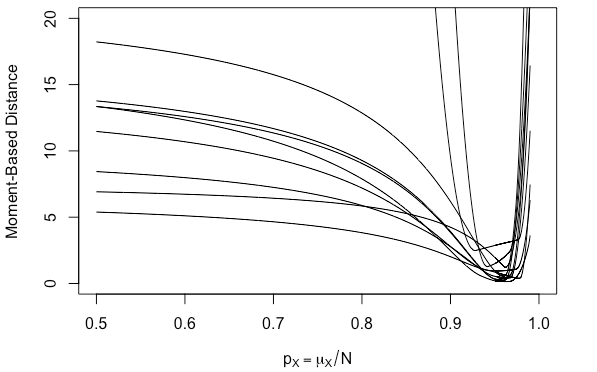
\includegraphics[width=\linewidth]{partial_plot.png}\\
    \captionof{Figure 2: }{Plots of $D(p_x) = min_{\boldsymbol{\pi}}D(p_x, \boldsymbol{\pi}).$}
\end{center}
\fi
}

\headerbox{Definitions}{name=def,span=1,column=0,below=intro}{
Each observed WRC score can be characterized as the sum of a true positive and a true negative score. Here, we define:\smallskip

$\rightarrow$ \textbf{True Positive Rate ($\boldsymbol{\pi_{tp}}$)}: The proportion of correctly read words that are accurately classified as correctly read by the scoring system.\smallskip

$\rightarrow$ \textbf{True Negative Rate ($\boldsymbol{1-\pi_{tn}}$)}: The proportion of incorrectly read words that are mistakenly classified as correctly read by the scoring system.\smallskip

We let $\boldsymbol{X}$ represent the \textbf{True Count Variable} -- a gold-standard measurement of the number of correctly read words in a passage consisting of $N$ words. The distribution of $X$ is assumed unknown with mean and variance $\mu_x$ and $\sigma_x^2$. \smallskip

To define the \textbf{Observed Count Variable}, we define \textbf{True Positive Score} Component
\begin{center}
\fbox{$$[X_1|X] \sim \text{Bin}(X, \pi_{tp})$$}  
\end{center}
and \textbf{True Negative Score} component
\begin{center}
\fbox{$$[X_2|X] \sim \text{Bin}(N-X, 1-\pi_{tn}).$$}  
\end{center}
The \textbf{Error-prone Count} is then given by 
\begin{center}
\fbox{$$Y=X_1 + X_2.$$}  
\end{center}

Two such error-prone counts can be realized. Let $\boldsymbol{Y_1}$ denote the \textbf{Score} observed by a \textbf{Human} assessor and let $\boldsymbol{Y_2}$ denote the \textbf{Score} recorded by the \textbf{AI} voice recognition software.\smallskip

Using the properties of the binomial distribution, as well as the properties of conditional expectations, we can quantify the relationships between gold-standard counts and error-prone counts.
}

\headerbox{Data Application}{name=app,span=1,column=3}{
The respective values of $\pi_{tn}$ and $\pi_{tp}$ were estimated from our data. The typical sample size is around $50$ measurements per passage; estimates are summarized in Table 2. Due to the restricted range of accuracy rates, we report truncated values, $\tilde{\pi}_{tp} = \min(\hat{\pi}_{tp}, 1)$ and $\tilde{\pi}_{tn} = \min(\hat{\pi}_{tn}, 1)$.
\begin{center}
    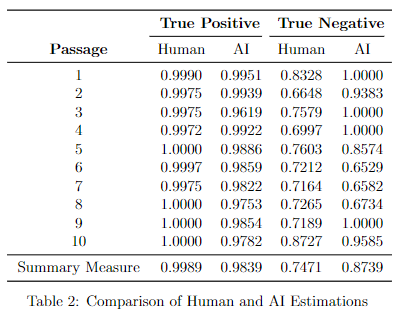
\includegraphics[width=1\linewidth]{compare.png}
\end{center}
}

\headerbox{Conclusion \& Future Works}{name=conc,span=1,column=3,below=app}{
Both human recorders and the AI systems demonstrate overall strong performance. Human recorders show higher consistency in True Positive values across passages while AI systems outperform human recorders in True Negative rates. %Both human recorders and AI systems record correct words read by students better than recording incorrect words.

\hfill 

In practice, gold-standard ORA measurements are unavailable. To this end, our next step will be to explore solutions assuming a statistical distribution for $X$. Then, defining $\hat{m} &= (\bar{y}_1, \bar{y}_2, s_1^2, s_2^2, s_{12})^\top$,
\vspace{-0.5\baselineskip}
\begin{align*}
\boldsymbol{\theta} & = (\mu_x,\pi_{tp1},\pi_{tp2},\pi_{tn1},\pi_{tn2})^\top, \ \text{and}\\
m(\boldsymbol{\theta}) &= (\mu_1(\boldsymbol{\theta}),\mu_2(\boldsymbol{\theta}),\sigma_1(\boldsymbol{\theta})^2,\sigma_2(\boldsymbol{\theta})^2, \sigma_{12}(\boldsymbol{\theta}))^\top,
\end{align*}

\vspace{-0.5\baselineskip}
we will estimate accurate rates by minimizing 
$D(\boldsymbol{\theta}) = (\hat{m} - m(\boldsymbol{\theta}))^\top \boldsymbol{\Sigma}^{-1} (\hat{m} - m(\boldsymbol{\theta})).$
}

\headerbox{References}{name=ref,span=1,column=3,below=conc}{

Nese, J. F. T., Kamata, A., \& Alonzo, J. (2015). Exploring the evidence of speech recognition and shorter passage length in computerized oral reading fluency. \textit{Paper presented at the Society for the Scientific Study of Reading meeting}, Kona, HI.
}


\end{poster}
\end{document}
